\section{Anforderungen}
\begin{itemize}
	\item Wenigstens ein Objekt in der Szene sollte bewegte Gliedmaßen haben.
	\item Wenigstens eine Szene sollte die Kameraeinstellung variieren, z.B. in die Szene hineinfahren, schwenken oder zoomen.
	\item Setzen Sie ein verarbeitetes Bild ein, z.B. als Höhenprofil, Kulisse oder Textur.
	\item Erstellen sie einen animierten Titel.
	\item Setzen Sie Überblendungen ein, um den Schnitt zwischen zwei Kamerapositionen oder anderen Bildwechseln zu betonen oder zu kaschieren.
	\item Setzen Sie Sound-Effekte zum Vertonen ein.
\end{itemize}
%
\section{Handlung}
Wir setzen ein Squashspiel in PovRay um. Die Spieler laufen durch den Gang in den Squashcourt, machen die Tür zu, geben sich die Hand und fangen an zu spielen. Nach ein paar Ballwechseln jubelt der eine Spieler und der Film ist zu Ende.
%
\section{Technisches}
\subsection{Grundlegendes und Konventionen}
\begin{itemize}
	\item Eine PovRay Distanzeinheit von $1.0$ entspricht $1.0$ Meter in der Realität
	\item Eine PovRay Clockeinheit von $1.0$ entspricht $1.0$ Sekunden in der Realität
	\item Das PovRay Koordinatensystem hat seinen Ursprung in der linken unteren hinteren Ecke des Squash Courts (siehe Grafik~\ref{fig:squashcourt} und \ref{fig:halloutline}).
\end{itemize}
%
\begin{figure}%[h!]
	\centering
	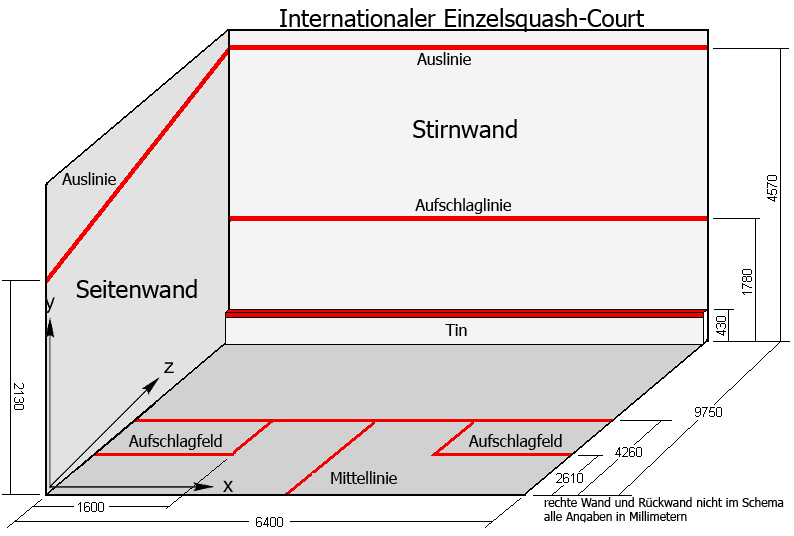
\includegraphics[width=.9\linewidth]{images/Squash_Court.png}
	\caption{Maße eines Squash Courts + PovRay Koordinatensystem}\label{fig:squashcourt}
\end{figure}
\begin{figure}%[h!]
	\centering
	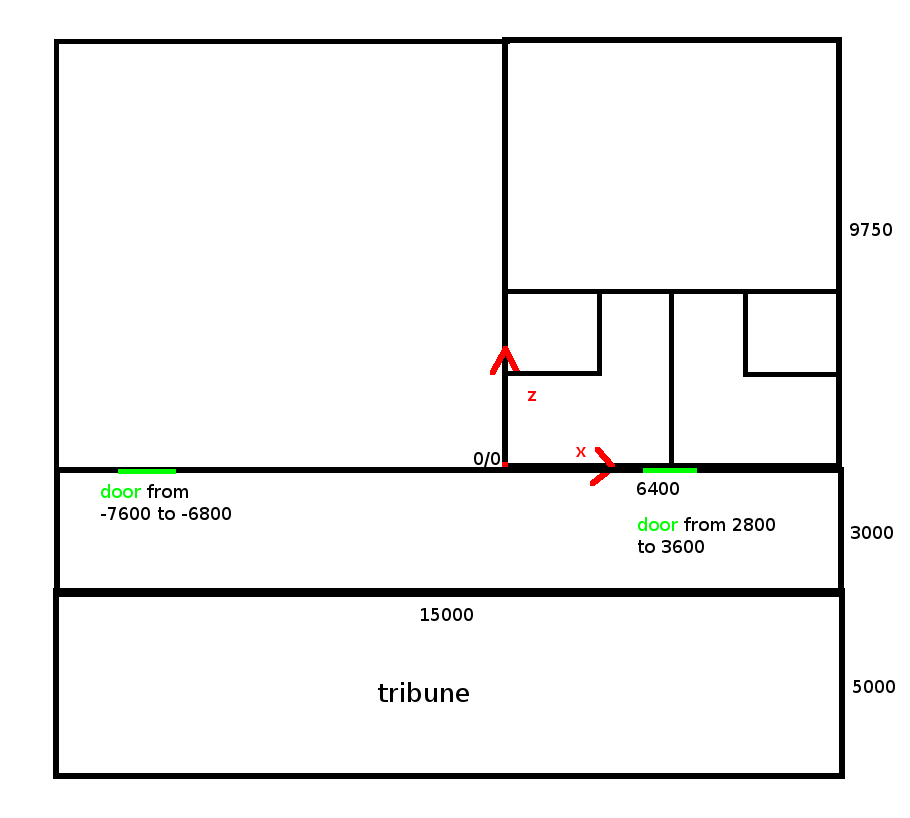
\includegraphics[width=.7\linewidth]{images/hall_outline.png}
	\caption{Grundriss der gesamten Karte}\label{fig:halloutline}
\end{figure}
\subsection{Aufbau des Programms}
TODO


